\label{chapter:desenvolvimento}
\section{Considerações Iniciais}
Neste capítulo expressa-se como foi vislumbrado um sistema de apoio didático ao ensino de programação, de que maneira foi modelado, 
quais decisões arquiteturais foram tomadas e como foi realizada sua implementação. Apresenta-se aqui uma visão geral do sistema, a visão específica que cada ator tem do sistema e a jornada de cada um desses usuários. De forma resumida, também é discutida a implementação das partes que compõem o sistema.
\section{Visão Geral}
O sistema \emph{Sharpener} foi construído para interagir com dois tipos de usuários; o Aluno e o Professor. O Professor pretende utilizar o \emph{Sharpener}
 em sala de aula, pois se interessa em ferramentas de apoio ao ensino e gostaria de acompanhar mais de perto a parte prática de suas aulas. O Aluno 
gostaria de utilizar ferramentas cômodas que o ajudassem no entendimento e resolução de exercícios.
% Quem são os atores do sistema? R: Professor e aluno

% Quais são os objetivos do professor no sistema? recuperar o plano 
% no Google Docs como redação (menos as partes que desistimos de fazer
Do ponto de vista do Professor, a ferramenta traz: a criação de um banco de exercícios, organizados por tópicos, 
de forma compartilhada entre professores; a possibilidade de inserção de dicas para auxiliar na resolução de exercícios; 
a possibilidade da elaboração de exercícios incrementais e um melhor acompanhamento do aluno levando em conta quais exercícios teve dificuldade. 
Do ponto de vista do Aluno, a ferramenta traz:  acesso a dicas, a opção de visualização da resposta do exercício e a substituição por exercício equivalente;
acesso a exercícios incrementais e uma forma 
simplificada de acesso e submissão de exercícios.

% Quais são os objetivos do aluno no sistema?
% recuperar plano, idem
O professor na plataforma é capaz de criar e gerenciar exercícios, trilhas e turmas. 
Alunos se inscrevem na plataforma por meio de um \emph{login} de identidade federada, e 
ingressam nas turmas por meio de um \emph{link} específico, que é fornecido 
pelo professor nos primeiros dias de aula. 

Trilhas de exercícios são preparadas por professores, que a associam às suas turmas. 
Estas trilhas são compostas de Grupos de Exercícios Equivalentes que 
contêm exercícios de assuntos correlatos e, idealmente, de mesmo nível de dificuldade.
Para cada aluno, é sorteado um exercício de cada grupo de forma aleatória. 
Caso o aluno apresente dificuldade na resolução deste exercício, o aluno pode solicitar 
dicas relativas ao exercício, ou, em último caso, a solução do mesmo. Caso a solução 
seja requisitada, outro exercício do mesmo Grupo de Exercícios Equivalentes é sorteado a este aluno.

Para diminuir o escopo inicial do projeto e incentivar o estudante a se familiarizar com o ferramental 
que envolve desenvolvimento de software, escolheu-se que o desenvolvimento do código 
acontecesse localmente no computador do aluno. Para que, ainda assim, proporcionemos ao aluno 
uma boa usabilidade do sistema, desenvolveu-se uma interface por linha de comando, que nos referiremos a partir de agora 
por \emph{CLI} (\emph{Command Line Interface}). Por meio desta \emph{CLI},
o aluno pode fazer \emph{downloads} e submissões
dos exercícios propostos de maneira rápida e prática.

Dessa forma, o sistema está dividido em três partes: uma interface gráfica, \emph{frontend}, 
em que professores e alunos possam interagir com exercícios, trilhas e turmas, uma \emph{CLI} que possibilita 
\emph{download} e submissão de exercícios, e um servidor com uma \emph{API} capaz de abstrair 
os recursos necessários por ambos os clientes. 

Na \fref{fig:arquitetura} apresenta-se um diagrama 
da arquitetura do sistema. Tanto a \emph{CLI} quanto o \emph{Frontend} se comunicam com o servidor através de sua \emph{API} \emph{Web} para que possa cumprir suas funcionalidades. A \emph{API} dispara funções no \emph{Backend} para que o recurso requisitado seja salvo ou recuperado. A maior parte dos dados do \emph{Backend} vem de uma conexão com o banco \emph{PostgreSQL}, hospedado no serviço \emph{Cloud SQL}. Apenas arquivos são salvos e recuperados através de requisições ao intervalo de armazenamento, chamado de \emph{Bucket}. 

  \begin{figure}[htpb]
    \centering
    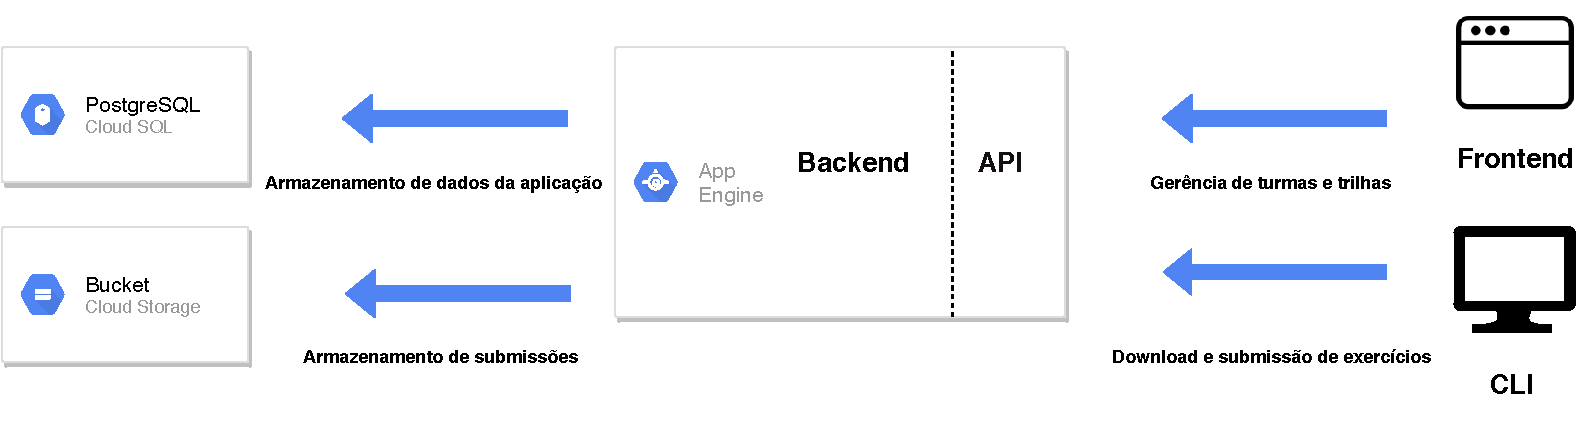
\includegraphics[width=\linewidth]{images/arquitetura.pdf}
    \caption{Arquitetura do sistema \emph{Sharpener}, o qual 
    se desenvolveu uma prova de conceito.}%
    \label{fig:arquitetura}
  \end{figure}
% Arquitetura resumida: a figura que já está pronta e o texto lá.

% Implementação, um resumo das linguagens e ferramentas 

\section{O sistema do ponto de vista do Aluno}
\label{ssec:aluno}

A rotina do Aluno no \emph{Sharpener} consiste em: ter acesso a um exercício, recorrer a alguma forma de apoio, completar o exercício submetendo uma versão, obter \emph{feedback}, e acompanhar seu andamento no curso. As principais atividades são realizadas na \emph{CLI}.

\subsection{Configuração}


O aluno tem acesso a uma interface de linha de comando, 
disponível para \emph{download} no \emph{Frontend}. Em seu primeiro 
acesso, o Aluno deve declarar que é o dono de uma \emph{token} que o identifica, isto é feito através do comando descrito em \cref{codigo:config}. A \emph{token} é obtida no \emph{Frontend}, depois de realizado o primeiro \emph{login}.

O aluno também deve ingressar na turma referente a seu professor, através de um \emph{link}, único para cada turma,
que será disponibilizado em sala de aula.

\begin{codigo}[caption={Configuração da CLI.}, label={codigo:config},language=bash, breaklines=true]
student@usp:~$ sharpener config <identificador-aluno>
\end{codigo}


\subsection{Acesso a exercícios}
Com a \emph{CLI} configurada, o aluno pode consultar 
se existem submissões pendentes. Para isto, deve recorrer ao 
comando descrito no \cref{codigo:list}. O comando invoca uma lista com todas as próximas submissões pendentes das trilhas em que está inscrito. Na listagem, cada submissão apresenta um identificador único.

\begin{codigo}[caption={Comando que lista submissões pendentes.}, label={codigo:list},language=bash, breaklines=true]
student@usp:~$ sharpener list
\end{codigo}

Com o identificador de submissão em mãos, o comando descrito em \cref{codigo:download} é utilizado para criar 
uma pasta com o nome do exercício no diretório que o comando foi invocado. Na pasta, todos os 
arquivos necessários para o desenvolvimento de uma solução estão presentes: descrição detalhada 
do problema, testes, um arquivo especificando dependências e um ponto de entrada.
Cada linguagem apresenta uma estrutura diferente de pastas, o \cref{codigo:pasta} mostra a execução 
do comando ``\emph{tree}'' que mostra como é a organização dos arquivos para a linguagem \emph{Rust}, no exercício \emph{accumulate}.
O aluno deve desenvolver sua solução no arquivo de ponto de entrada, 
que no exemplo anterior, se encontra em ``src/lib.rs''.

\begin{codigo}[caption={Download de exercício pela \emph{CLI}.}, label={codigo:download},language=bash, breaklines=true]
student@usp:~$ sharpener download <identificador-exercicio>
\end{codigo}

\newpage
\begin{codigo}[caption = {Estrutura de pasta para um exercício em Rust}, label={codigo:pasta},language=bash, breaklines=true]
student@usp~$ tree
    Cargo.toml
    README.md
    src
        lib.rs
    tests
        accumulate.rs
2 directories, 5 files

\end{codigo}

% explicar a consulta na CLI (não existe, vamos desenhar/projetar)
% explicar o download na CLI

\subsection{Apoio a resolução de exercício}
Para que o aluno consiga evoluir sua solução até uma que esteja correta, testes automatizados estão presentes 
nos exercícios disponíveis no \emph{Sharpener}. Com o comando descrito em \cref{codigo:test}, os testes são 
executados e impressos no terminal. Caso todos os testes forem cumpridos, o código está pronto para submissão, do contrário 
mudanças devem ser feitas no código e repete-se o processo.

\begin{codigo}[caption = {Executando a bateria de testes a partir da \emph{CLI}.}, label={codigo:test},language=bash, breaklines=true]
student@usp:~$ sharpener test 
\end{codigo}

% Buscando dicas
Caso o professor deseje disponibilizar dicas acerca do exercício, o Aluno pode invocar o comando descrito no \cref{codigo:hint}. 
Uma nova dica será mostrada no terminal, guiando o Aluno na resolução do exercício.

\newpage
\begin{codigo}[caption = {Comando para solicitar dicas do exercício na \emph{CLI}.}, label={codigo:hint},language=bash, breaklines=true]
student@usp:~$ sharpener hint
\end{codigo}

% Buscando/obtendo a resposta final
O Aluno, em último caso, pode desistir de resolver aquele exercício em específico do Grupo de Exercícios Equivalentes. 
O comando descrito em \cref{codigo:solution}, após uma confirmação do aluno, faz \emph{download} de um arquivo contendo uma possível 
solução. Quando o comando é emitido, é registrado que aquele exercício do Grupo de Exercícios Equivalentes foi pulado e um novo exercício é 
baixado e colocado no diretório pai do exercício atual. A desistência só é possível se houver outro exercício disponível no Grupo de Exercício Equivalentes.

Para que a submissão seja válida o arquivo de testes deverá ser idêntico ao que foi baixado. Caso 
este contenha modificações, a \emph{CLI} notificará o aluno que este é o caso e abortará a submissão.
\begin{codigo}[caption = {Comando para requisitar a solução de um exercício na \emph{CLI}}, label={codigo:solution},language=bash, breaklines=true]
student@usp:~$ sharpener solution
\end{codigo}



% Buscando/obtendo um Exercício Equivalente/Alternativo

\subsection{Submissão de resposta}
% 
Se a solução desenvolvida pelo Aluno cumprir todos os testes, sua submissão é possível. Com o comando descrito por \cref{codigo:submit}, 
sua solução é enviada, juntamente com o \emph{output} dos testes. Caso o comando seja invocado e os testes ainda não estão sendo cumpridos, um 
alerta notifica o Aluno que este é o caso, e o questiona se deseja continuar mesmo assim. Múltiplas tentativas de submissão podem ser feitas, 
sendo todas elas salvas pelo sistema. Assume-se que a última submissão é a que deve ser corrigida, mas o professor, se desejar, pode inspecionar tentativas feitas anteriormente.

\begin{codigo}[caption = {Comando para submeter exercícios na \emph{CLI}}, label={codigo:submit},language=bash, breaklines=true]
student@usp:~$ sharpener submit
\end{codigo}

%\subsection{Exercícios incrementais}

%\subsection{Acompanhamento do andamento na disciplina}

\section{O sistema do ponto de vista do Professor} 
\label{ssec:professor}
\subsection{Gerenciando turmas e trilhas}
A jornada do professor também começa no \emph{Frontend}, que tem sua página inicial descrita pela \fref{fig:login}.
Após seu \emph{login} pelo \emph{Github}, este deve informar a um administrador 
do sistema que sua conta precisa ser elevada a condição de professor, já que todas as contas são alunos por \emph{default}.

  \begin{figure}[htb]
    \centering
    
\includegraphics[width=\linewidth]{images/mocks/login.png}
    \caption{Página de \emph{Login} da prova de conceito do sistema \emph{Sharpener}.}%
    \label{fig:login}
  \end{figure}

Assim que o Professor fizer \emph{login} na plataforma, o Professor é direcionado para página de turmas, como podemos visualizar na \fref{fig:turmas}. 
Este deve criar sua primeira turma, dando a ela um nome único, como mostra a \fref{fig:turmasAdd}. 

 \begin{figure}[htpb]
    \centering
    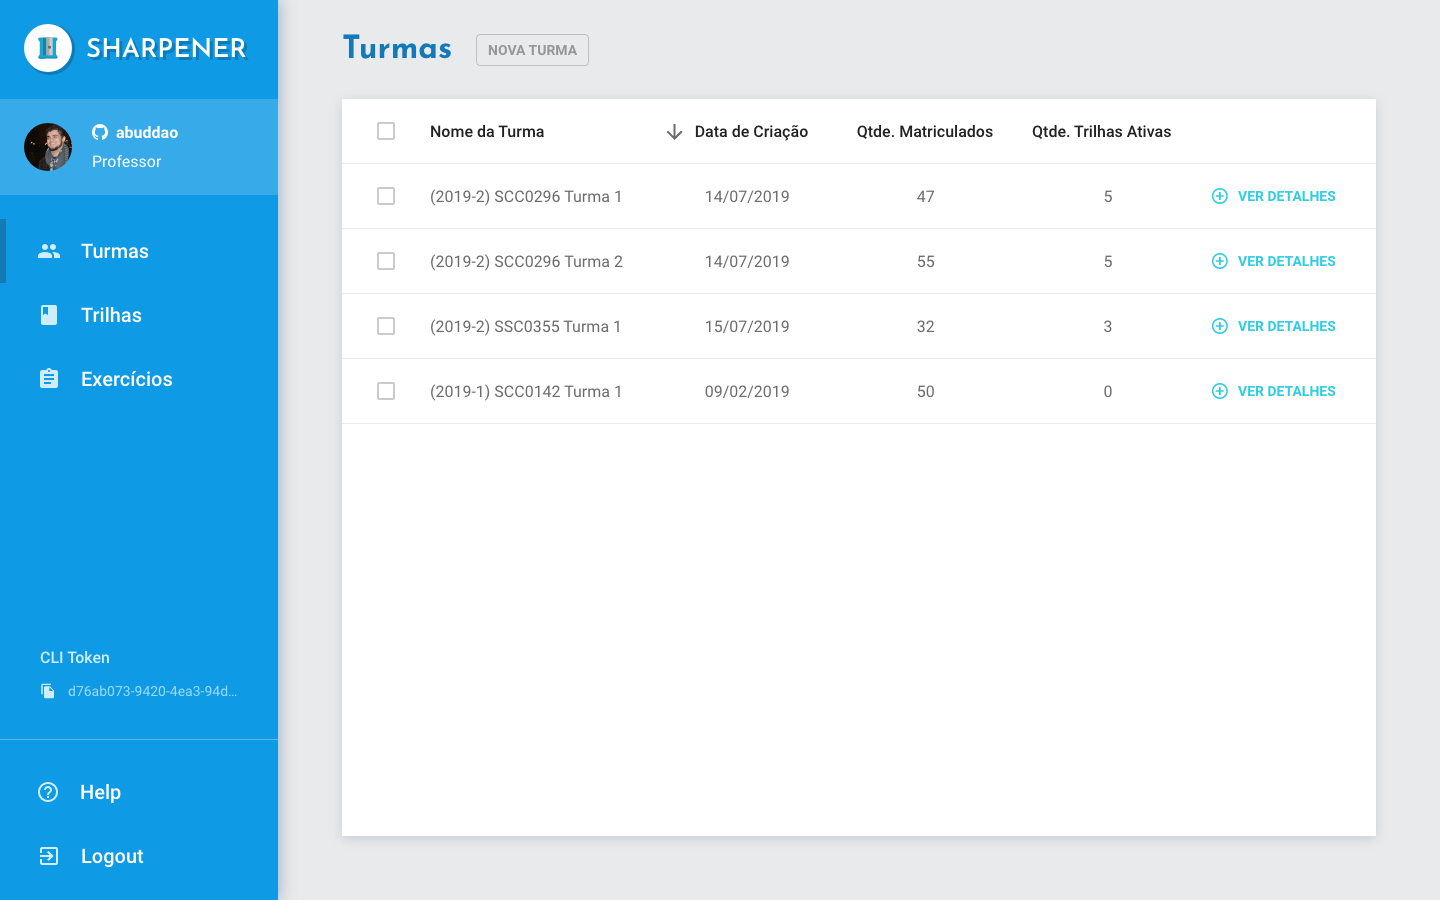
\includegraphics[width=\linewidth]{images/mocks/turmaExpandido.png}
    \caption{Página de turmas da prova de conceito do sistema \emph{Sharpener}.}%
    \label{fig:turmas}
  \end{figure}
  
    \begin{figure}[htpb]
    \centering
    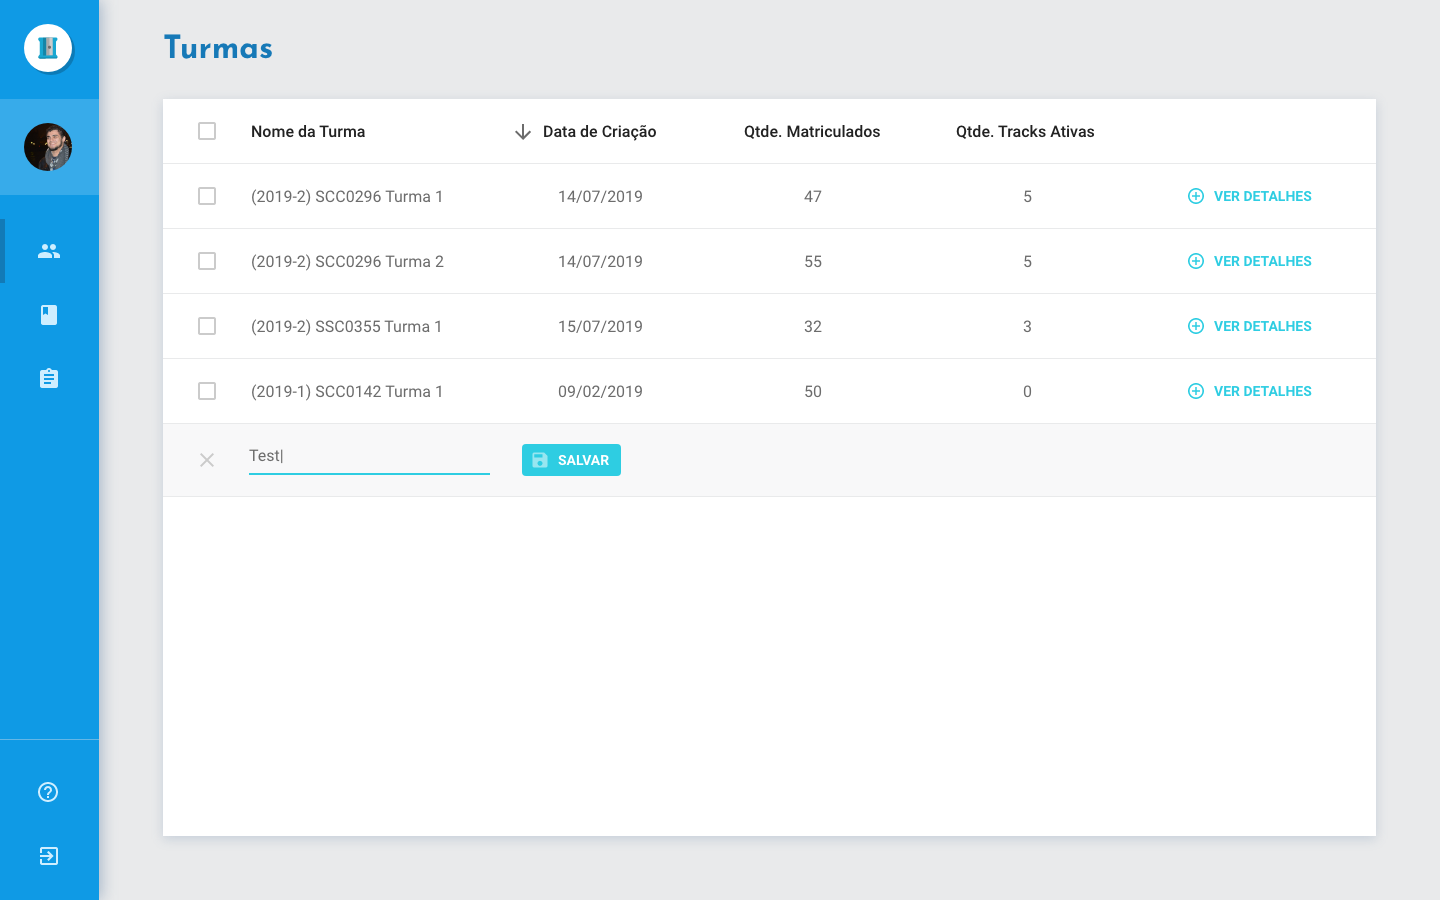
\includegraphics[width=\linewidth]{images/mocks/turmaNova.png}
    \caption{Página de turmas da prova de conceito do sistema \emph{Sharpener}, em que se 
    cria uma nova turma.}%
    \label{fig:turmasAdd}
  \end{figure}

O próximo passo é a criação de uma trilha de exercícios, que pode ser feita na página descrita pela \fref{fig:track}. Cada trilha
contém Grupos de Exercícios Equivalentes. O professor associa exercícios 
a cada um destes grupos, podendo filtrá-los por nome na barra superior direto. 
Tal sequência é mostrada pela \fref{fig:add_track1}, \fref{fig:add_track2}, \fref{fig:add_track3} e \fref{fig:add_track4}.  

  \begin{figure}[htb]
  \centering
  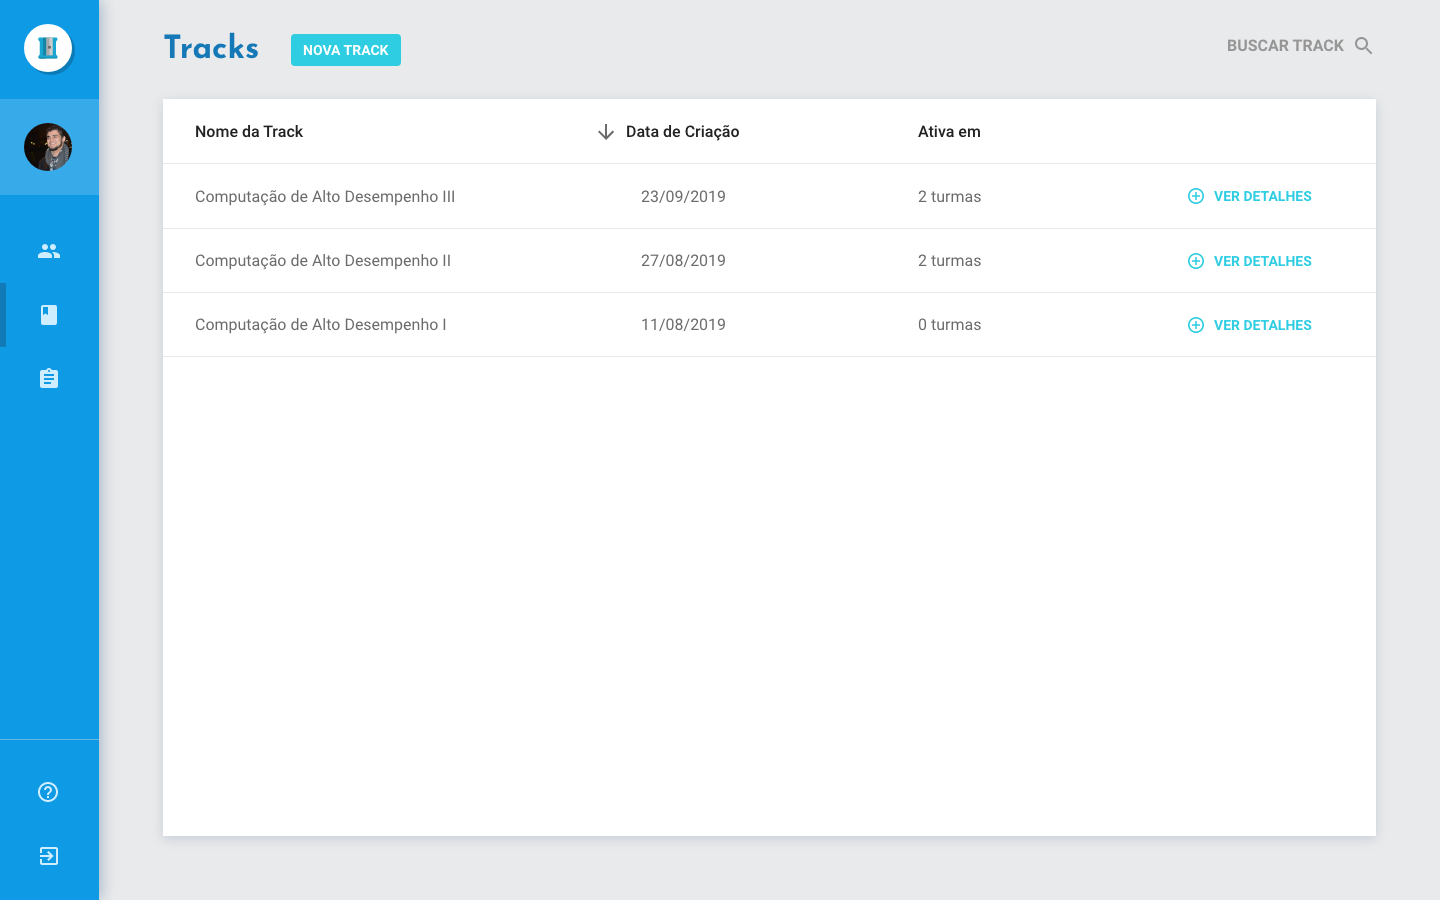
\includegraphics[width=\linewidth]{images/mocks/track.png}
  \caption{Página de trilhas da prova de conceito do sistema \emph{Sharpener}.}%
  \label{fig:track}
  \end{figure}
  
    \begin{figure}[htpb]
  \centering
  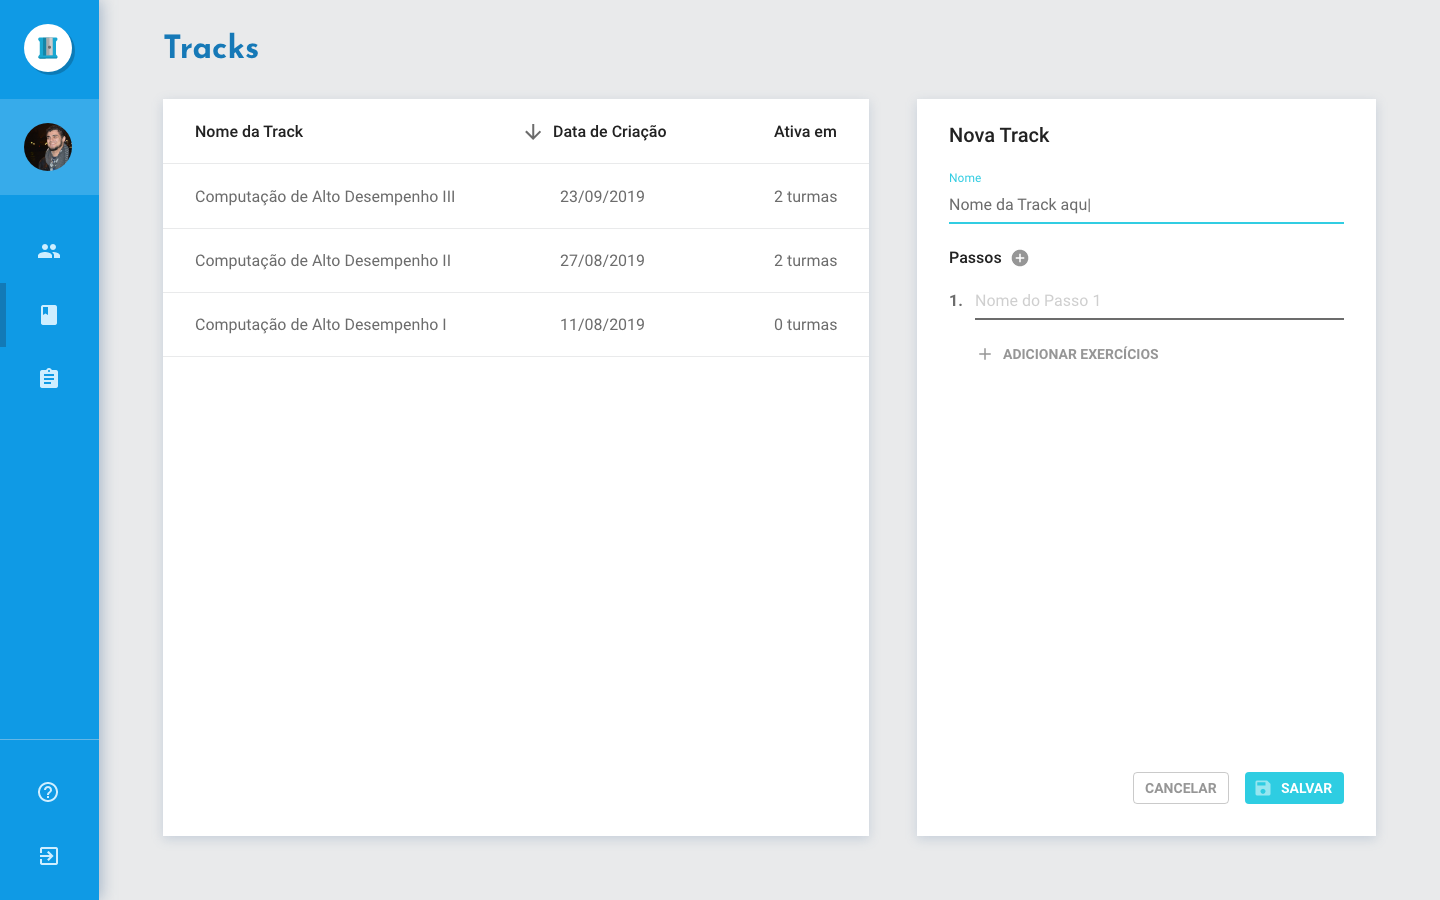
\includegraphics[width=\linewidth]{images/mocks/trackAdd1.png}
  \caption{Página de trilhas da prova de conceito do sistema \emph{Sharpener}, 
  em que uma nova trilha é criada.}%
  \label{fig:add_track1}
  \end{figure}
  
    \begin{figure}[htpb]
  \centering
  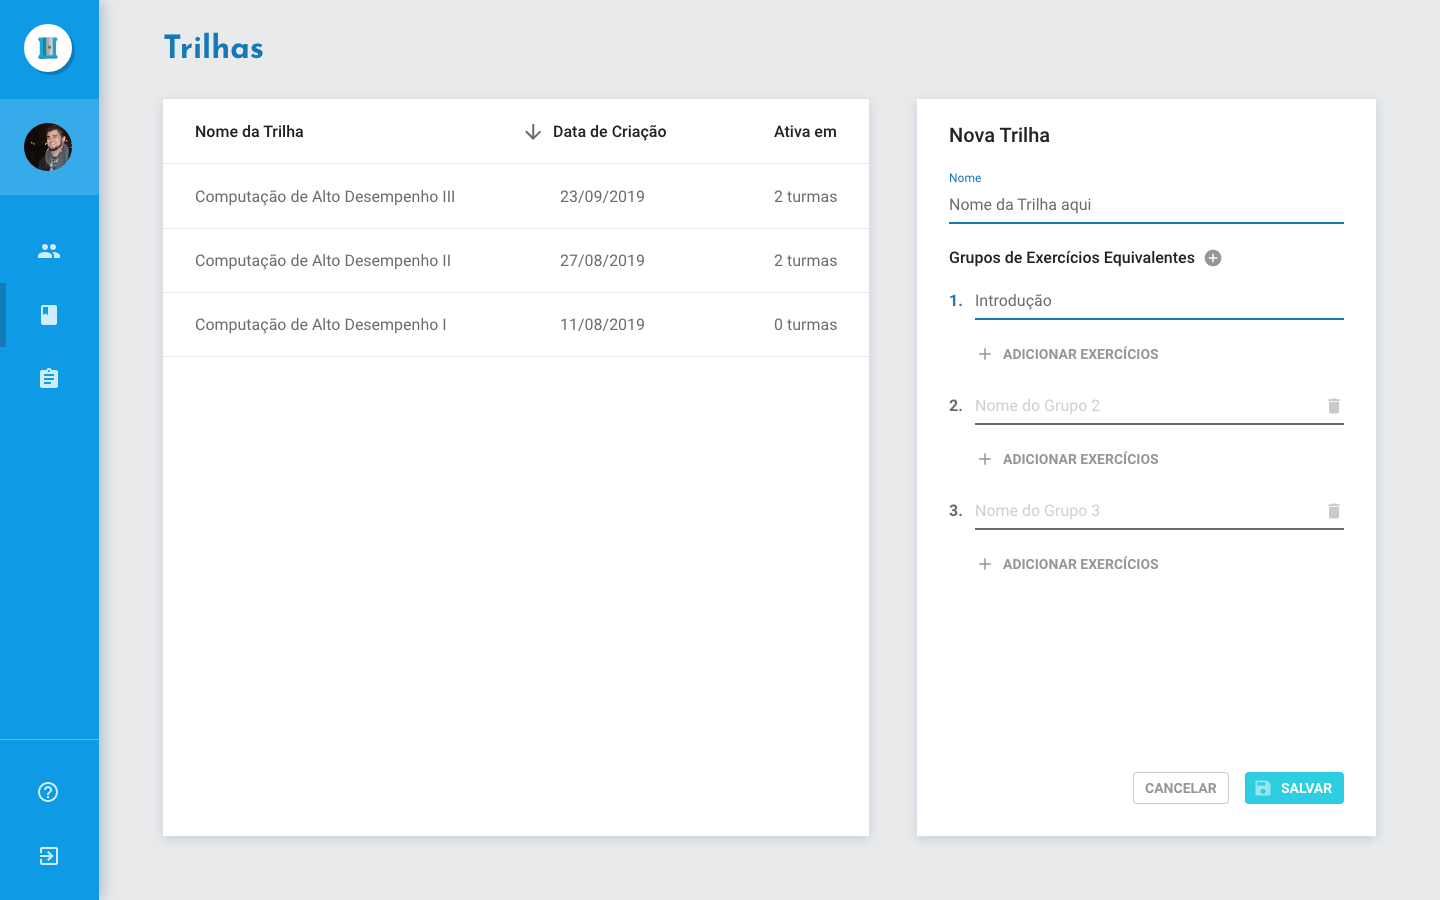
\includegraphics[width=\linewidth]{images/mocks/trackAdd2.png}
  \caption{Página de trilhas da prova de conceito do sistema \emph{Sharpener}, 
  em que novos Grupos de Exercícios Equivalentes são criados.}%
  \label{fig:add_track2}
  \end{figure}

  \begin{figure}[htpb]
  \centering
  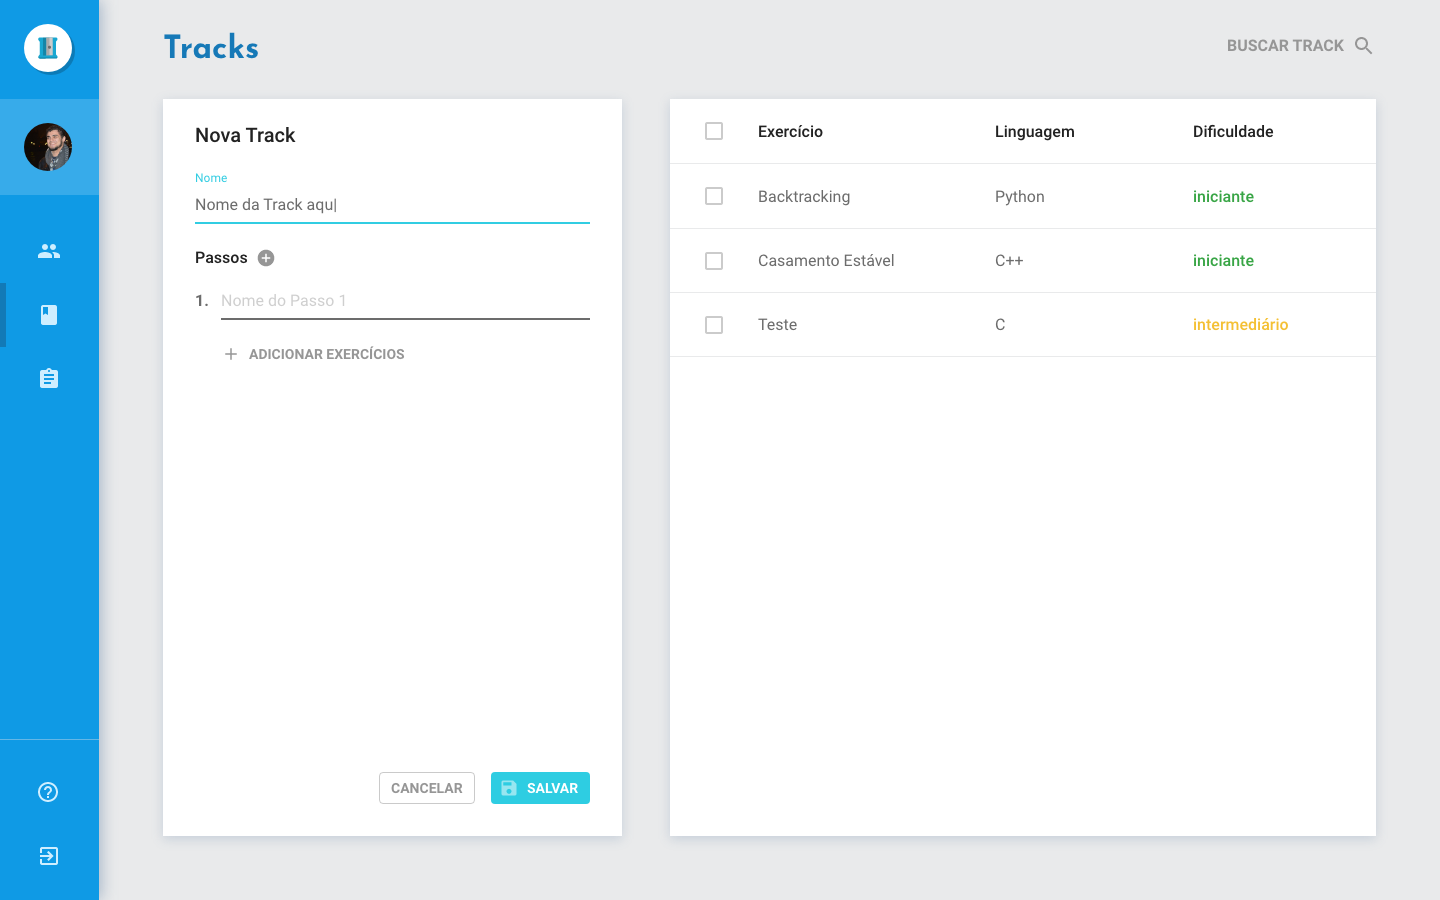
\includegraphics[width=\linewidth]{images/mocks/trackAdd3.png}
  \caption{Página de trilhas da prova de conceito do sistema \emph{Sharpener}, 
	  em que Grupos de Exercícios Equivalentes são associados a passos de uma trilha, parte 1.}%
  \label{fig:add_track3}
  \end{figure}
  
  \begin{figure}[htpb]
  \centering
  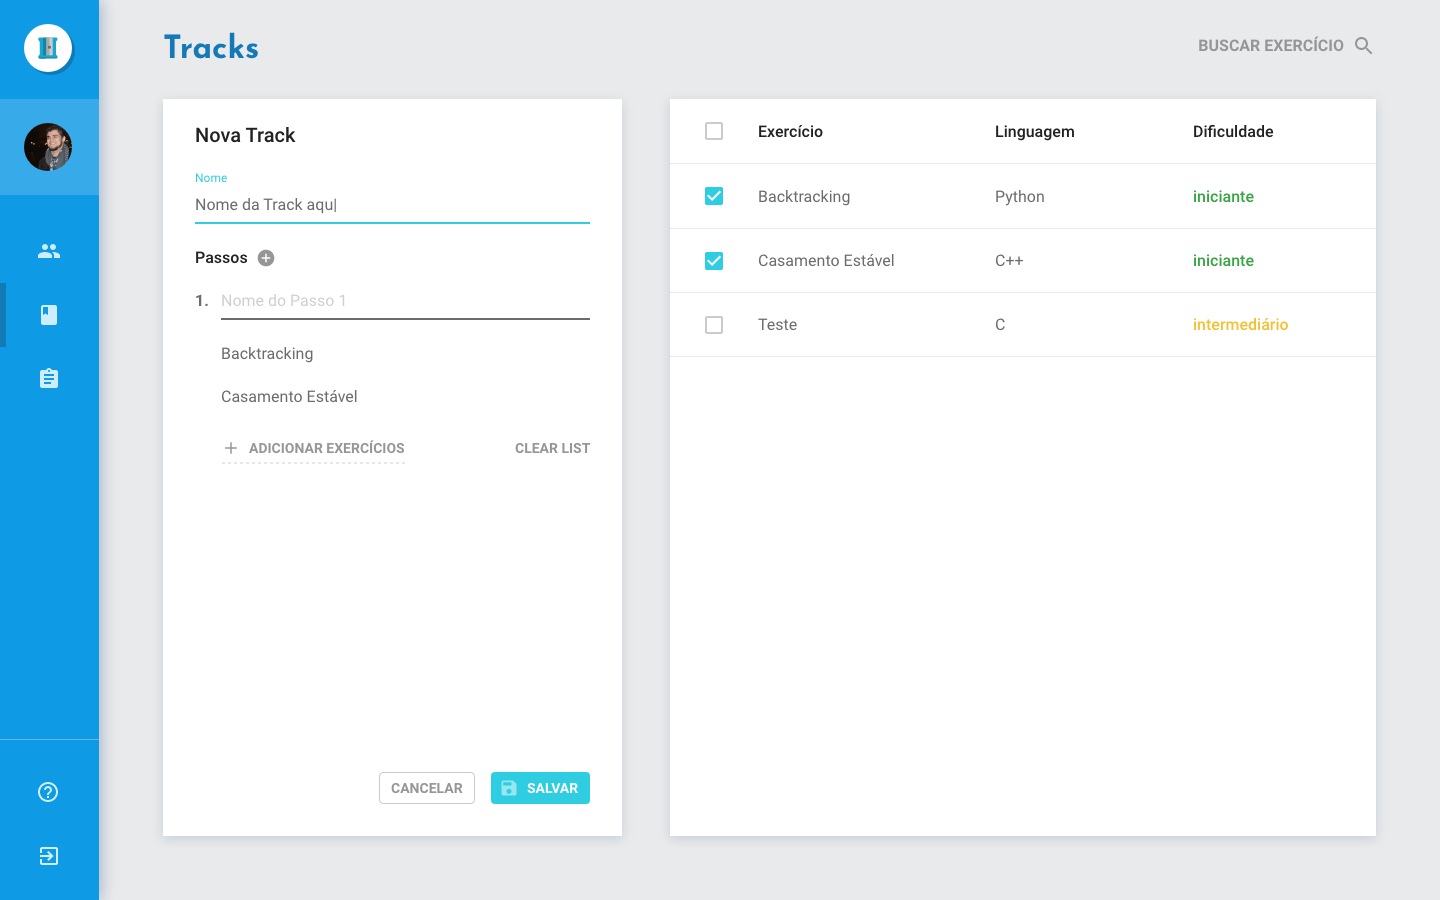
\includegraphics[width=\linewidth]{images/mocks/trackAdd4.png}
  \caption{Página de trilhas da prova de conceito do sistema \emph{Sharpener}, 
	  em que Grupos de Exercícios Equivalentes são associados a passos de uma trilha, parte 2.}%
  \label{fig:add_track4}
  \end{figure}

Caso o professor ainda não tenha definido todos os exercícios que compõem sua trilha, uma visita a página de exercícios pode lhe 
ser útil. A página conta com todos os exercícios disponíveis no banco de exercícios que podem ser filtrados por nomes ou tópicos, 
como pode ser visto pela \fref{fig:exercicios}.

  \begin{figure}[htb]
  \centering
  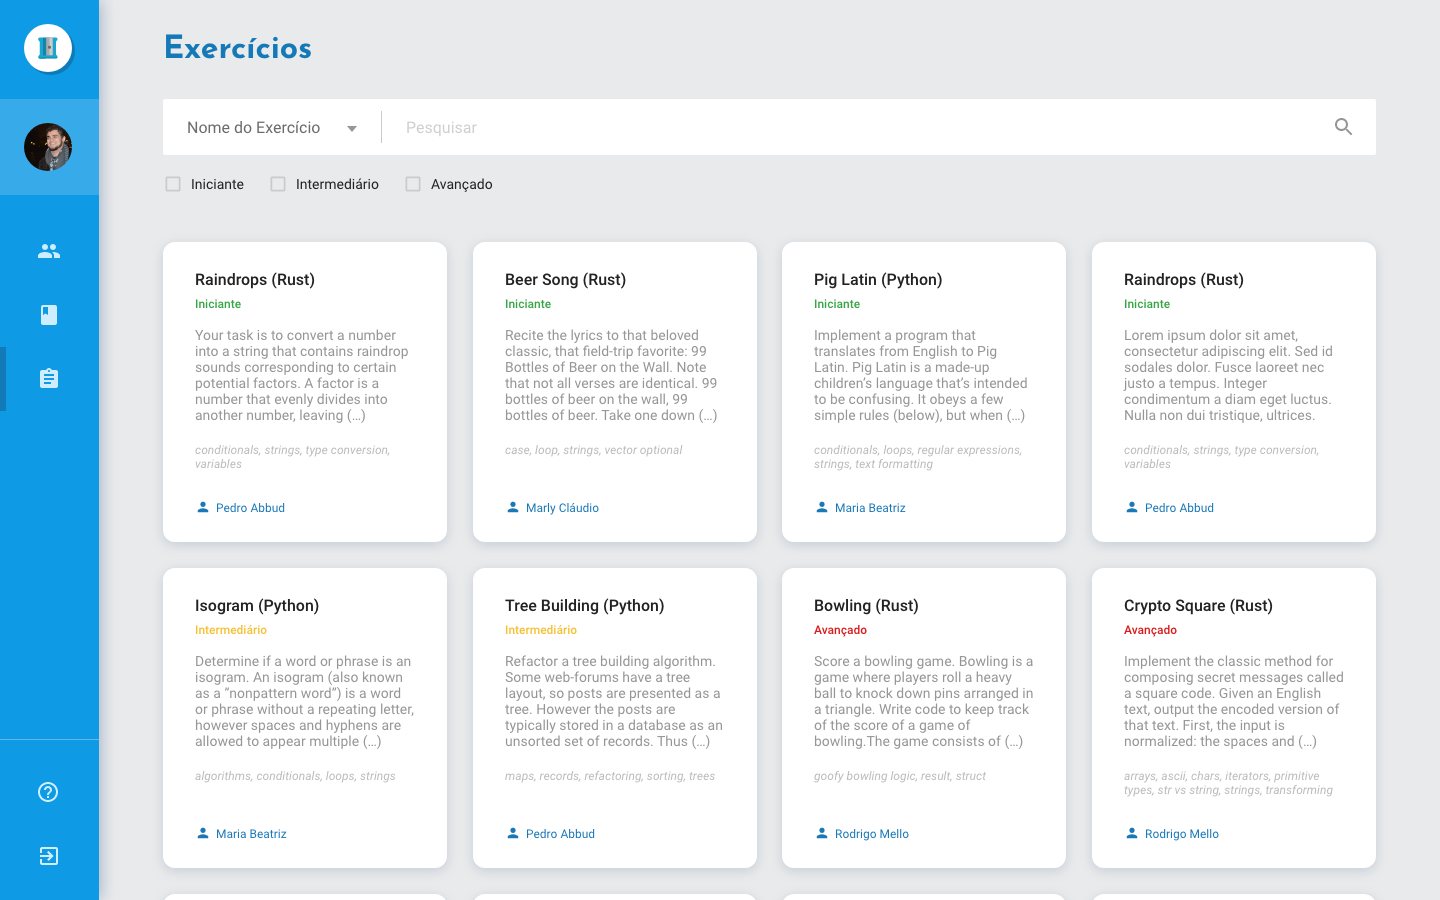
\includegraphics[width=\linewidth]{images/mocks/exercicios.png}
  \caption{Página de exercícios da prova de conceito do sistema \emph{Sharpener}.}%
  \label{fig:exercicios}
  \end{figure}

O passo final é associar a trilha recém criada às suas turmas. Isto pode ser feito voltando na página de turmas, selecionando 
turmas e clicando no botão ``Adicionar \emph{Track}''. Um modal cobre a tela e é possível selecionar e procurar trilhas, dentre 
as disponíveis, para associar a estas turmas. A \fref{fig:enroll_track1} e \fref{fig:enroll_track2} mostram esta interação.

  \begin{figure}[htb]
    \centering
    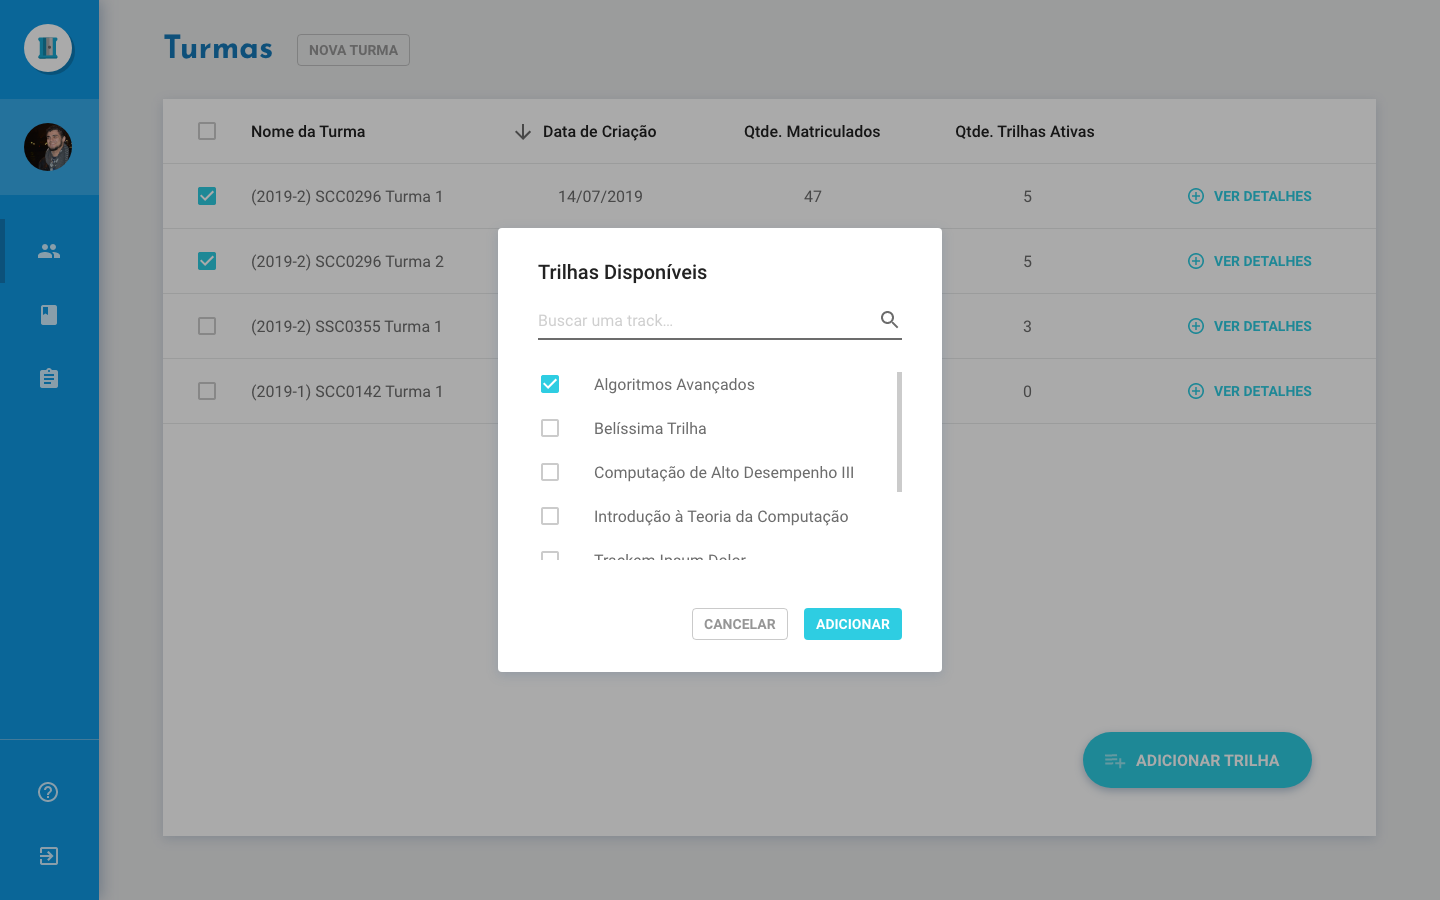
\includegraphics[width=\linewidth]{images/mocks/turmaAddTrack.png}
    \caption{Página de turmas da prova de conceito do sistema \emph{Sharpener}, em 
	    que o professor inscreve suas turmas em trilhas.}%
    \label{fig:enroll_track1}
  \end{figure}
  
    \begin{figure}[htb]
    \centering
    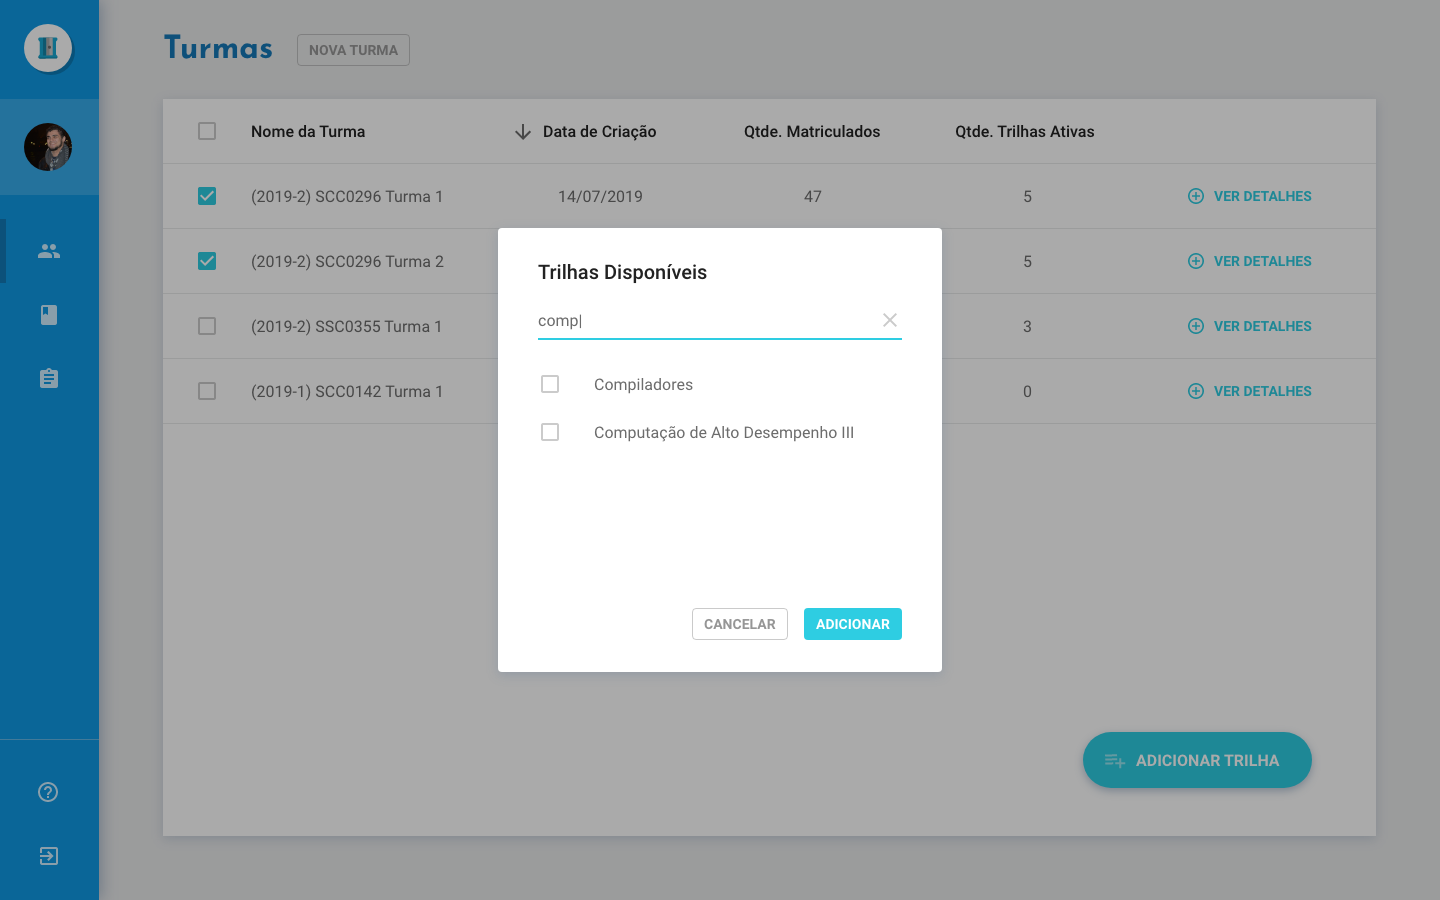
\includegraphics[width=\linewidth]{images/mocks/turmaAddTrackSearch.png}
    \caption{Página de turmas da prova de conceito do sistema \emph{Sharpener}, 
    que o professor inscreve suas turmas em trilhas, com um filtro  aplicado.}%
    \label{fig:enroll_track2}
  \end{figure}


% Preparar e carregar exercícios
\subsection{Preparando exercícios}
% \Sref já coloca Seção
Para a preparação de novos exercícios que farão parte do banco de exercícios, o professor precisa
ter baixado, instalado e configurado a \emph{CLI}, da mesma forma descrita na \Sref{ssec:aluno}. Há um comando para criar um novo exercício. Nesse caso, o Professor deve invocar o comando com a sintaxe descrita em \cref{codigo:new}. Este comando criará um diretório novo diretório com os arquivos 
que deverão ser preenchidos pelo professor antes de submeter o exercício para o banco 
de exercícios. Os arquivos a serem preenchidos são: um arquivo chamado ``README.md'', contendo as instruções 
do que se espera no exercício, um arquivo contento testes, outro arquivo que conterá código produzido pelo aluno 
e um arquivo que contém uma solução para o exercício, escrito pelo professor.

\begin{codigo}[caption = {Comando para criar novos exercícios na \emph{CLI}}, label={codigo:new},language=bash, breaklines=true]
prof@usp:~$ sharpener exercise new <language> <exercise_name>

\end{codigo}

Se o Professor desejar adicionar dicas para o exercício, este deve preencher o arquivo escondido,
``.meta.json''. A chave \emph{``hints''} deve conter um \emph{Array} de \emph{Strings}, em que 
cada uma delas é uma dica. O campo ``topics'' deste mesmo arquivo pode ser preenchido para relacionar 
este exercício a estes tópicos.

Para submeter o exercício criado o professor deve executar o comando descrito por \cref{codigo:post} na 
pasta que contém o exercício.

\begin{codigo}[caption = {Comando para submeter novos exercícios na \emph{CLI}}, label={codigo:post},language=bash, breaklines=true]
prof@usp:~$ sharpener exercise post
\end{codigo}

Caso deseje alterar um exercício, poderá baixá-lo através do comando \cref{codigo:download_prof} e 
ressubmetê-lo pelo \cref{codigo:post}. Apenas professores estão autorizados a utilizar o 
\cref{codigo:download_prof} e ressubmissões só podem ser feitas por exercícios de autoria daquele 
professor.
\begin{codigo}[caption = {Comando para baixar exercícios em modo edição na \emph{CLI}}, label={codigo:download_prof},language=bash, breaklines=true]
prof@usp:~$ sharpener exercise download <language> <exercise_name>

\end{codigo}



%% Enunciados
%% Casos de teste
%% Dicas
%% Grupo de Exercícios Equivalentes/Alternativos
%\subsubsection{Exercícios incrementais}
Como trilhas contêm Grupos de Exercícios Equivalentes, que serão resolvidos de forma sequencial pelo aluno, 
é possível propor exercícios incrementais. O efeito é atingido montando Grupos de Exercícios Equivalentes que contenham apenas um exercício. Assim, o aluno não pode pedir outro exercício equivalente e 
deve passar naquela trilha por todos os incrementos propostos.

% Acompanhar uma turma ou um aluno
\newpage

\section{A \emph{API} (\emph{Application Programming Interface})}
\subsection{Especificação}
Para suprir as necessidades da \emph{CLI} e do 
\emph{Frontend}, a \emph{API Web} fornece vários recursos diferentes. Alguns destes recursos não são protegidos, enquanto outros necessitam de identificação, que é provida pelo seu token pessoal. Os recursos disponíveis são
descritos a seguir, em que nomes entre o símbolo de maior e menor significam nomes variáveis 
da \emph{URI}.
\begin{description}
\item[\texttt{/api/classes}]  Rota protegida que, se o usuário for um professor, mostra todas as turmas que este criou. Caso o usuário seja aluno, mostra todas as classes em que faz parte. 
Aceita apenas o método \emph{GET}.
\item[\texttt{/api/classes/<name>}] Rota protegida que aceita apenas o método \emph{PUT}, emitido por 
um professor. Cria uma turma com o nome especificado. Turmas de um mesmo professor precisam 
ter nomes diferentes.
\item[\texttt{/api/classes/<name>/<track>}] Rota protegida que permite apenas o método \emph{PUT}, emitido por 
um professor. Associa uma turma, identificada pelo nome e criado por este mesmo professor, em uma determinada trilha.
\item[\texttt{/api/enrollments/<invite\_token>}] Rota protegida que aceita apenas o método \emph{POST}. Inscreve o Aluno em determinado turma, identificada por um código de convite.
\item[\texttt{/api/exercises}] Rota que aceita apenas o método \emph{GET}. Lista exercícios do banco 
de exercícios, por ordem ascendente por nível de dificuldade. A rota aceita paginação por meio 
de duas \emph{query strings}: ``\emph{page\_size}'' e ``\emph{page}''.
\item[\texttt{/api/exercises/<language>}] Rota que aceita apenas o método \emph{GET}. Lista exercícios do banco 
de exercícios, que sejam da linguagem especificada, por ordem ascendente por nível de dificuldade. A rota aceita paginação por meio 
de duas \emph{query strings}: ``\emph{page\_size}'' e ``\emph{page}''.
\item[\texttt{/api/exercises/<language>/<name>}] Rota protegida que aceita os método \emph{GET} e
\emph{PUT}. Ao receber um méotodo \emph{GET}, de um professor, mostra todos os detalhes relativos ao exercício, como a descrição do problema e \emph{URI}s para download dos artefatos associados. Se o ponto de acesso receber um \emph{PUT}, cria ou atualiza o exercício no banco de exercícios. Exercícios só podem ser atualizados se o criador do exercício foi o professor emissor da requisição.
\item[\texttt{/api/submissions/<submission\_token>}] Rota protegida que aceita  métodos \emph{POST} e \emph{GET}. O método \emph{GET} retorna todos os detalhes do exercício relativa a submissão referenciada 
por um \emph{token} de submissão e o método \emph{POST} registra uma tentativa de submissão.
\item[\texttt{/api/submissions/<submission\_token>/forfeit}] Rota protegida que aceita  métodos \emph{POST}.
Uma submissão nesta rota informa ao sistema que o estudante desiste da resolução deste exercício. A rota 
devolve a solução do exercício e uma \emph{token} de submissão de um novo exercício do mesmo Grupo de Exercícios Equivalentes. A desistência só será aceita se houver um novo exercício do Grupo de Exercícios Equivalentes, o qual o aluno ainda não tentou resolver.
\item[\texttt{/api/topics}] Rota que aceita apenas o método \emph{GET}. Mostra todos os tópicos já abordados por exercícios do banco de exercícios.
\item[\texttt{/api/topics/<language>}] Rota que aceita apenas o método \emph{GET}. Mostra todos os tópicos já abordados por exercícios do banco de exercícios, filtrados pela língua que foi 
provida na \emph{URI}.
\item[\texttt{/api/tracks/<track\_name>}] Rota protegida que aceita apenas o método \emph{PUT} de Professores. 
Cria uma nova trilha com o nome indicado na \emph{URI}, contanto que o professor não tenha criado outra com este mesmo nome.
\item[\texttt{/api/tracks/<track\_name>/classes/<class\_name>}] Rota protegida que aceita apenas o método \emph{PUT} de Professores. Matricula todos os alunos 
presentes na turma, que ainda não foram matriculados, na trilha que foi associada a uma turma específica. Ao invocar este ponto de acesso, o sistema cria 
, para cada aluno naquela turma e cada Grupo de Exercícios Equivalentes, uma submissão em estado pendente. Cada submissão é associada a um exercício aleatoriamente 
escolhido do Grupo de Exercícios Equivalentes. Se novos Alunos ingressarem na turma e uma nova requisição for disparada  ao ponto de acesso, submissões serão apenas 
criadas aos novos Alunos.
\item[\texttt{/api/healthcheck}] Rota que aceita apenas o método \emph{GET}. Informa se o serviço está funcionando corretamente e se a conexão com o banco de dados foi comprometida. Esta rota foi feita para que uma sonda externa faça esta consulta, e que caso haja alguma anormalidade, que um novo contêiner da aplicação seja iniciado e o tráfego direcionado a ele. 
\end{description}

Fora da \emph{API}, existem duas outras rotas, criadas especificamente para o \emph{Frontend}.
A primeira delas está exposta na raiz do servidor e serve o \emph{template} contendo o código da  \emph{single page application} do \emph{Frontend}. Uma outra rota, servida em ``\texttt{/authenticate}'', também se fez necessária para ser possível autenticação do usuário pelo \emph{Github}. A rota salva na sessão do usuário que está logado e suas informações, para que a maior parte dos acessos futuros não necessitem repetir os passos de autenticação federada.
% Pontos de acesso, etc. etc.

\subsection{Implementação} % DA API
A implementação do protótipo do servidor foi desenvolvida na linguagem \emph{Python} em conjunto 
com o \emph{microframework Web}, \emph{Flask}. Escolheu-se o banco de dados relacional \emph{PostgreSQL} para armazenamento dos dados e a \emph{ORM} \hyperref[link:sqlalchemy]{\emph{SQLAlchemy}}  para mapear 
o esquema do banco de dados em classes. 

Pela comodidade e confiabilidade, escolheu-se utilizar um serviço de computação em nuvem ao invés de rodar o projeto \emph{On-Premisses}. A \emph{Cloud} escolhida foi a \hyperref[link:gcp]{\emph{Google Cloud Plataform}}. 
Fez-se uso do serviço de armazenamento de intervalos para salvar arquivos de exercícios e submissões,
e do \hyperref[link:appengine]{\emph{AppEngine}}, o  \emph{Platform as a Service} da provedora, para hospedar a aplicação.
% Discutir o protótipo do servidor: repassar as opções de cloud, banco, etc

Detalhes de implementação estão detalhadas no \Aref{chapter:implementacao}. Os repositórios dos três projetos, \emph{API Web},  \emph{CLI} e \emph{Frontend} são de domínio público, e são de código aberto, aceitando assim contribuições de interessados.

\section{Resultados}
Um protótipo de sistema foi desenvolvido, conforme discutido anteriormente. Nesta versão alfa, testaram-se \emph{workflows} básicos 
como as sequências discutidas nas \Sref{ssec:aluno} e \Sref{ssec:professor}; em resumo foi testado a interação com turmas, trilhas e exercícios. Os \emph{endpoints} presentes na \emph{API} pareceram suficientes para as atividades  
propostas e a \emph{CLI} provou-se uma forma interessante do Aluno interagir com a plataforma. Nem todo o \emph{design} do \emph{frontend} foi, de fato, implementado. Como o foco do projeto foi, principalmente, o desenvolvimento da \emph{CLI} e da \emph{API Web},  apenas a parte vital para execução dos fluxos anteriores foi desenvolvida.

Para os testes na versão alfa foram extraídos exercícios de outra plataforma, \emph{exercism}. Através de um \emph{script}, de forma automática, inseriu-se diversos exercícios no banco de dados. 222 exercícios, de duas linguagens diferentes, compuseram o conjunto extraído, exercícios os quais tiveram 157 tópicos distintos associados a eles. Com esta variedade de exercícios, pôde-se ter uma ideia de como o sistema se comportaria em versões futuras.
